\documentclass[tikz]{standalone}
\usetikzlibrary{arrows.meta}
\begin{document}

\begin{tikzpicture}[-latex, arrows={-Triangle[angle=20:5pt,scale=1.5]}]
	\node (X) at (0,0) {};
	\node (A1) at (3,0) {\(A\)};
	\node (A2) at (0,-3) {\(A\)};
	\node (B) at (3,-3) {\(B\)};
	\fill (X) circle (2pt);
	\draw (X) to node [above] {\(u\)} (A1);
	\draw (X) to node [left] {\(v\)} (A2);
	\draw (A1) to node [right] {\(f\)} (B);
	\draw (A2) to node [below] {\(f\)} (B);
\end{tikzpicture}

\begin{tikzpicture}[-latex, arrows={-Triangle[angle=20:5pt,scale=1.5]}]
	\node (X) at (0,0) {};
	\node (A1) at (3,0) {\(A\)};
	\node (A2) at (0,-3) {\(A\)};
	\node (B) at (3,-3) {\(B\)};
	\node (C) at (5,-5) {\(C\)};
	\fill (X) circle (2pt);
	\draw (X) to node [above] {\(u\)} (A1);
	\draw (X) to node [left] {\(v\)} (A2);
	\draw (A1) to node [right] {\(f\)} (B);
	\draw (A2) to node [below] {\(f\)} (B);
	\draw (B) to node [above right] {\(g\)} (C);
\end{tikzpicture}

\begin{tikzpicture}[scale=0.7,-latex, arrows={-Triangle[angle=20:5pt,scale=1.5]}]
	\node (X) at (0,0) {};
	\node (A1) at (3,0) {\(A\)};
	\node (A2) at (0,-3) {\(A\)};
	\node (B1) at (6,0) {\(B\)};
	\node (B2) at (0,-6) {\(B\)};
	\node (C) at (6,-6) {\(C\)};
	\fill (X) circle (2pt);
	\draw (X) to node [above] {\(u\)} (A1);
	\draw (X) to node [left] {\(v\)} (A2);
	\draw (A1) to node [above] {\(f\)} (B1);
	\draw (A2) to node [left] {\(f\)} (B2);
	\draw (B1) to node [right] {\(g\)} (C);
	\draw (B2) to node [below] {\(g\)} (C);
\end{tikzpicture}

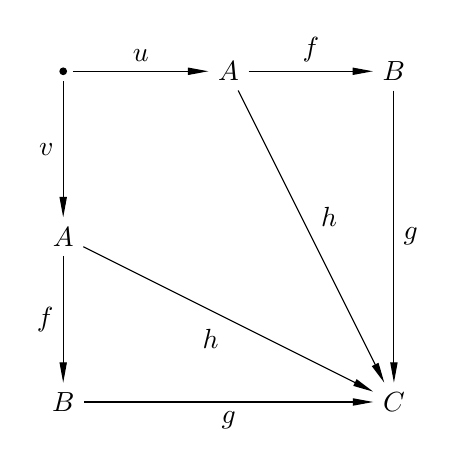
\begin{tikzpicture}[scale=0.7,-latex, arrows={-Triangle[angle=20:5pt,scale=1.5]}]
	\node (X) at (0,0) {};
	\node (A1) at (3,0) {\(A\)};
	\node (A2) at (0,-3) {\(A\)};
	\node (B1) at (6,0) {\(B\)};
	\node (B2) at (0,-6) {\(B\)};
	\node (C) at (6,-6) {\(C\)};
	\fill (X) circle (2pt);
	\draw (X) to node [above] {\(u\)} (A1);
	\draw (X) to node [left] {\(v\)} (A2);
	\draw (A1) to node [above] {\(f\)} (B1);
	\draw (A2) to node [left] {\(f\)} (B2);
	\draw (B1) to node [right] {\(g\)} (C);
	\draw (B2) to node [below] {\(g\)} (C);
	\draw (A1) to node [above right] {\(h\)} (C);
	\draw (A2) to node [below left] {\(h\)} (C);
\end{tikzpicture}

\begin{tikzpicture}[-latex, arrows={-Triangle[angle=20:5pt,scale=1.5]}]
	\node (X) at (0,0) {};
	\node (A1) at (3,0) {\(A\)};
	\node (A2) at (0,-3) {\(A\)};
	\node (C) at (3,-3) {\(C\)};
	\fill (X) circle (2pt);
	\draw (X) to node [above] {\(u\)} (A1);
	\draw (X) to node [left] {\(v\)} (A2);
	\draw (A1) to node [right] {\(h\)} (C);
	\draw (A2) to node [below] {\(h\)} (C);
\end{tikzpicture}

\begin{tikzpicture}[-latex, arrows={-Triangle[angle=20:5pt,scale=1.5]}]
	\node (X) at (0,0) {};
	\node (A1) at (3,0) {\(A\)};
	\node (A2) at (0,-3) {\(A\)};
	\fill (X) circle (2pt);
	\draw (X) to node [above] {\(u\)} (A1);
	\draw (X) to node [left] {\(v\)} (A2);
	\draw (A1) to node [below right] {\(1_A\)} (A2);
\end{tikzpicture}

\end{document}
